\section{Algorithm}
\label{sec:algorithm}
\subsection{Line Segment Intersection}
\label{sec:line_segment_intersection}
A naive approach to line segment intersection is to compare each pair of segments for intersection. This approach has a time complexity of $O(n^2)$ where $n$ is the number of line segments.

In the worse case scenario where all line segments intersect with each other the lower bound for the time complexity is $\Omega(n^2)$ because all intersections must be reported but in real cases scenarios we usually have that a line segment intersects only a small set of other segments. We want an algorithm that performs better that the naive approach in these more common cases. This type of algorithms where the complexity depends not only on the input size but also on the input itself are called \textit{output-sensitive algorithms}.

The algorithm we implemented is based on the \textit{sweep line} paradigm. The idea is to move a horizontal line from top to bottom while keeping track of the segments currently intersecting the line in a \textit{status} structure. The status is updated only at specific \textit{event points} where the line intersects a segment.

The algorithm uses two main data structures: the \textit{event queue} and the \textit{status structure}. The event queue is a priority queue that contains all the event points sorted by their $y$ coordinate. The status structure is a balanced binary search tree that contains all the segments intersecting the sweep line sorted by their $x$ coordinate.

The algorithm works as follows:
\begin{enumerate}
    \item Initialize the event queue with all the endpoints of the segments.
    \item While the event queue is not empty:
          \begin{enumerate}
              \item Pop the event point with the largest $y$ coordinate from the event queue.

                    \begin{minipage}{0.6\textwidth}
                        \item If the event point is the upper endpoint of a new segment $s$:
                        \begin{enumerate}
                            \item Insert $s$ in the status structure.
                            \item Check if $s$ intersects the segment to its left $s_l$ and the one to its right $s_r$ in the status structure.
                        \end{enumerate}
                    \end{minipage}
                    \hfill
                    \begin{minipage}{0.3\textwidth}
                        \centering
                        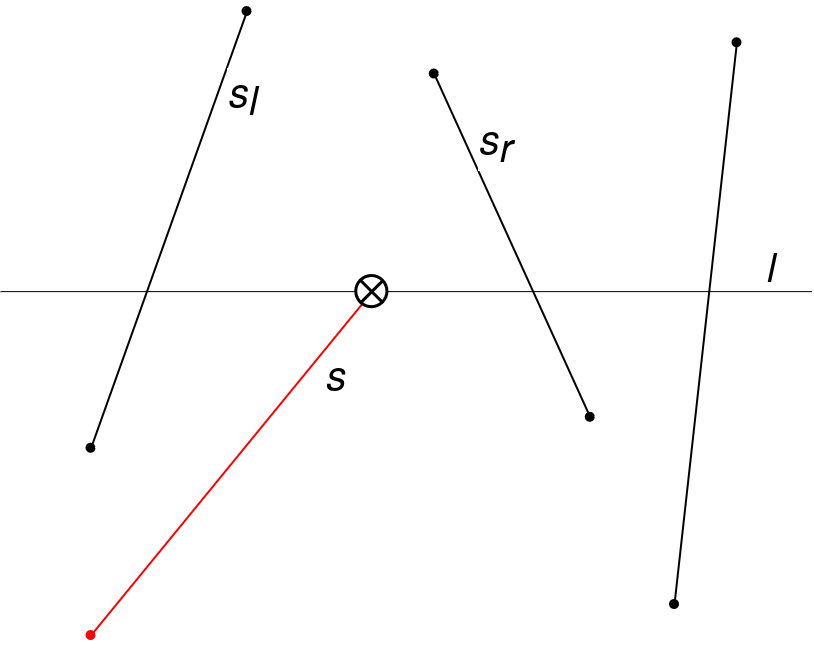
\includegraphics[width=\textwidth]{images/upper.png}
                    \end{minipage}
                    \hfill \break
                    \begin{minipage}{0.6\textwidth}
                        \item If the event point is the lower endpoint of a segment $s$:
                        \begin{enumerate}
                            \item Remove $s$ from the status structure.
                            \item Check if the segments to the left and to the right of $s$ ($s_l$ and $s_r$ respectively) which are now adjacent in the status structure intersect.
                        \end{enumerate}
                    \end{minipage}
                    \hfill
                    \begin{minipage}{0.3\textwidth}
                        \centering
                        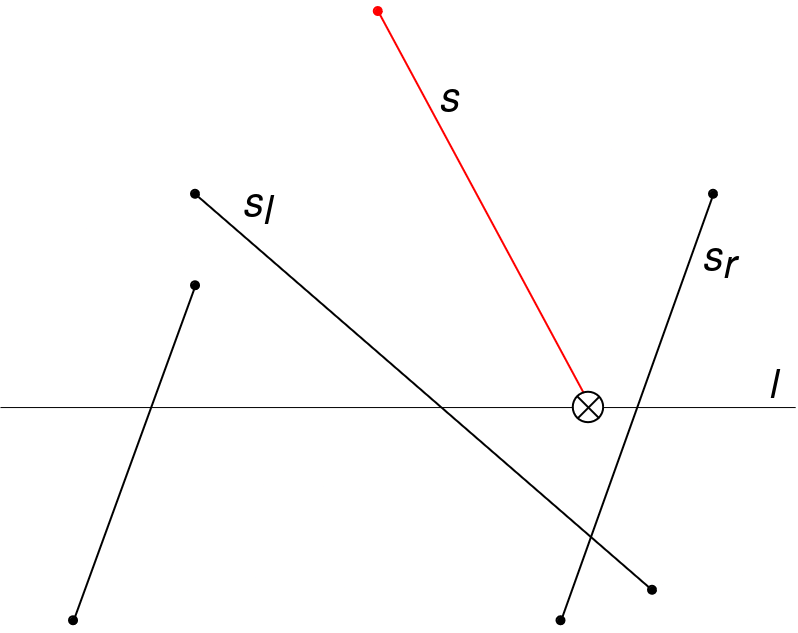
\includegraphics[width=\textwidth]{images/lower.png}
                    \end{minipage}
                    \hfill \break
                    \begin{minipage}{0.6\textwidth}
                        \item If the event point is an intersection point between two segments $s_1$ and $s_2$:
                        \begin{enumerate}
                            \item Report the intersection.
                            \item Swap the positions of $s_1$ and $s_2$ in the status structure.
                            \item Assuming $s_1$ is now to the left of $s_2$, test them for intersection with their new neighbors. For $s_1$ this eans testing for intersection with the segment to its left ($s_l$) and for $s_2$ testing for intersection with the segment to its right ($s_r$).
                        \end{enumerate}
                    \end{minipage}
                    \hfill
                    \begin{minipage}{0.3\textwidth}
                        \centering
                        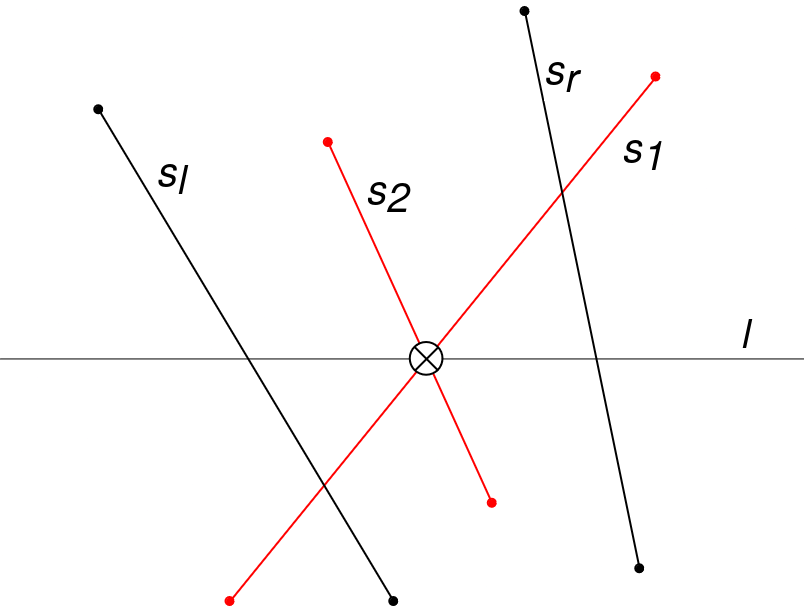
\includegraphics[width=\textwidth]{images/intersection.png}
                    \end{minipage}
          \end{enumerate}
\end{enumerate}

We can check that a segment is intersecting exclusively with the segments to its left and to its right because the segments in the status structure are sorted by their $x$ coordinate and if two segments intersect at some point they must have no segments between them and thus they must be adjacent in the status structure.

The time complexity of this algorithm is $O(n\log n + m \log n)$ where $n$ is the number of segments and $m$ is the number of intersections. The first term comes from the sorting of the event queue and the second term comes from the operations on the status structure that are all $O(\log n)$ and are performed for each intersection.


\subsection{Doubly Connected Edge List}
\label{sec:dcel}
The overlay task consists in computing the intersection of two planar subdivisions. The algorithm we implemented is derived from the \textit{sweep line} algorithm for line segment intersection described above.

The first step is to define a data structure that represents the planar subdivision. We chose to use the \textit{Doubly Connected Edge List} (DCEL) data structure because it allows us to easily represent the planar subdivision as a set of vertices, edges and faces and to perform operations on it.
\hfill \break
\begin{minipage}{0.5\textwidth}
    \centering
    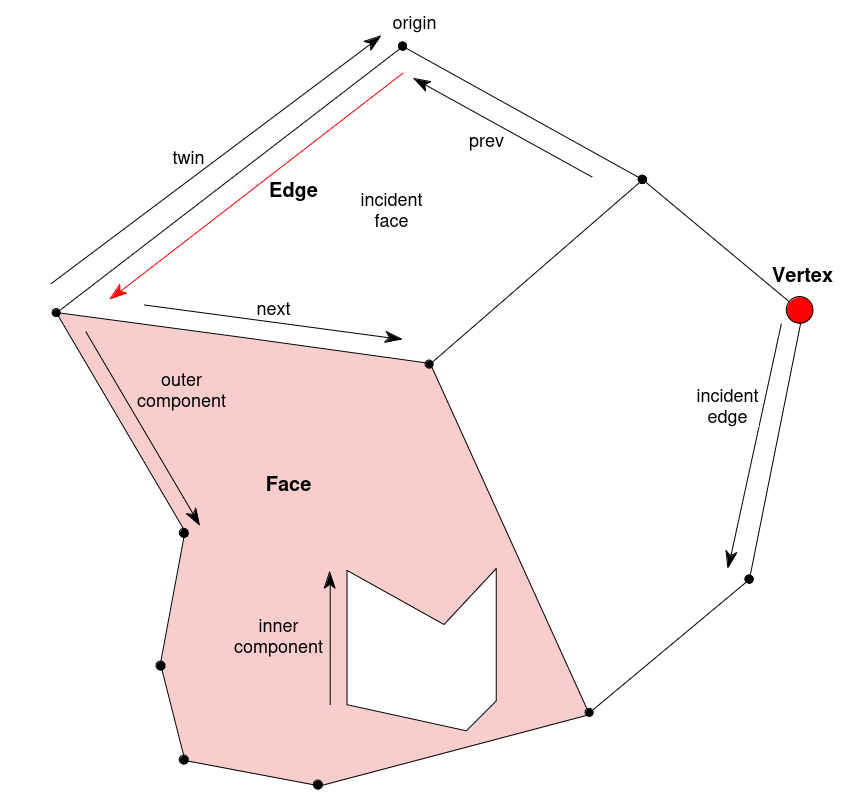
\includegraphics[width=\textwidth]{images/dcel.png}
\end{minipage}
\begin{minipage}{0.5\textwidth}
    \begin{itemize}
        \item Vertex: each vertex stores its coordinates and a pointer to one of the half-edges that starts at that vertex.
        \item Edge: each edge stores a pointer to its origin vertex, a pointer to its twin edge, a pointer to the previous and to the next edge in the boundary to and a pointer to the face it belongs to. We don't need to store the destination vertex because its equal to the origin of its twin edge.
    \end{itemize}
\end{minipage}
\begin{itemize}
    \item Face: each face stores a pointer to one of the half-edges that bounds it (this pointer is null for the unbounded face). This edge is chosen so that the face it bounds is always on its left side which implies we traverse the face in counter-clockwise order.It also stores a list of pointers to a half-edge for each hole in the face. Differently from the outer boundary, the holes are stored in clockwise order so that the face they bound is still on their left side.
\end{itemize}

\subsection{Overlay of Two Subdivisions}
\label{sec:overlay}
\noindent \textit{Overlay}: we define the overlay of two planar subdivisions $S_1$ and $S_2$ to be the planar subdivision $S$ such that there is a face $f$ in $S$ if and only if there are faces $f_1$ in $S_1$ and $f_2$ in $S_2$ such that $f = f_1 \cap f_2$ is maximal. More simply, the overlay is the intersection of the two subdivisions.

We create the DCEL for the overlay by first copying the vertices and edges of the two input DCELs. The edges from the original subdivisions that don't intersect any other edge don't need to be modified while the edges that intersect other edges from a different subdivision need to be split at the intersection points.

Starting from the sweep line algorithm for line segment intersection we can easily extend it to compute the overlay of two subdivisions. The algorithm works as follows:
\begin{enumerate}
    \item Initialize the event queue with all the endpoints of the edges of the two subdivisions.
    \item While the event queue is not empty:
          \begin{enumerate}
              \item Pop the event point with the largest $y$ coordinate from the event queue.
              \item Update the status structure as in the line segment intersection algorithm.
              \item If the event point is an intersection point between edges from different subdivisions we need to split the edges at the intersection point and update the DCEL. Three main cases can happen:
                    \begin{enumerate}
                        \item The intersection point is an endpoint for all intersecting edges
                        \item The intersection point is an endpoint only for the edges belonging to one of the two subdivisions
                        \item The intersection point is an interior point for all intersecting edges
                    \end{enumerate}
          \end{enumerate}
\end{enumerate}

\begin{minipage}{0.3\textwidth}
    \centering
    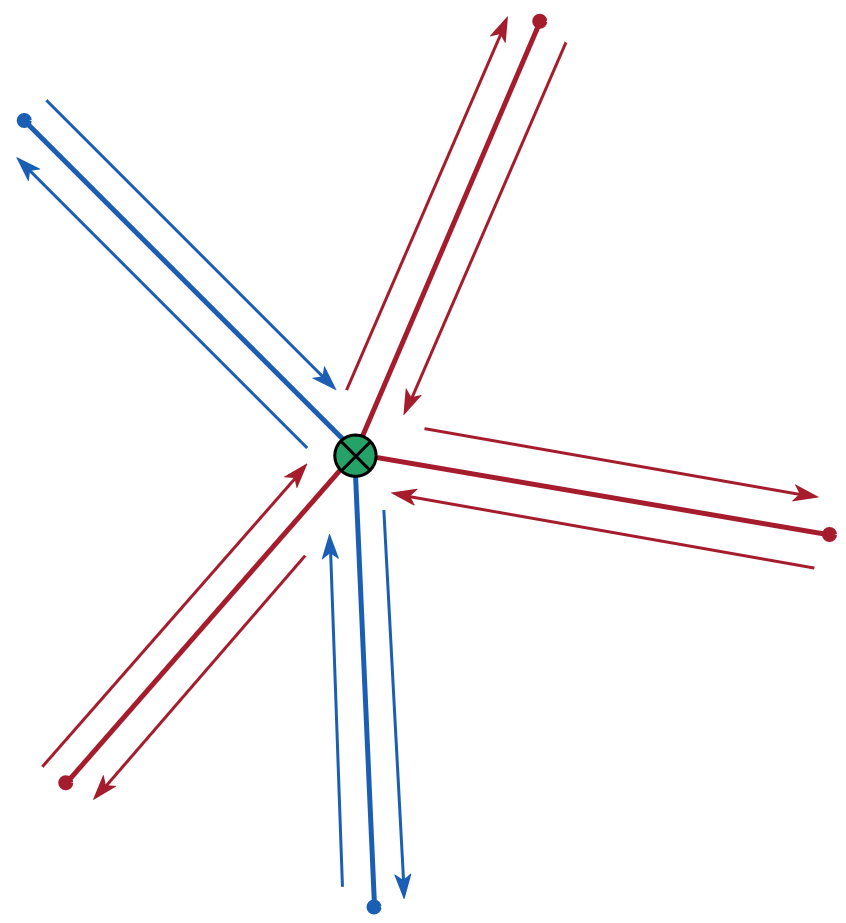
\includegraphics[width=0.9\textwidth]{images/vertex.png}
\end{minipage}\hfill
\begin{minipage}{0.7\textwidth}
    The first case is the simplest because no edge needs to be split and no vertex has to be added to the DCEL. The only thing we need to do is update the pointers of the edges around the intersection point $v$ so that they point to the correct edges: the prev pointer for each of the incident edges of $v$ must point to the twin of the first incident edge of $v$ seen in counter-clockwise order. Respectively, the next pointer for each of the incident edges twins must point to the first incident edge of $v$ seen in clockwise order.
\end{minipage}
\break


\begin{minipage}{0.7\textwidth}
    Assuming the intersection point is an endpoint only for the edges of the first subdivision, we need to split the edge $e$ from the second subdivision into two edges $e^{\prime}$ and $e^{\prime\prime}$ both with the intersection point $v$ as origin together with their corresponding twins.

    We need to update the pointers around the endpoints of the original edge $e$: the next pointers of the two new half-edges $e^{\prime}$ and $e^{\prime\prime}$ each copy the next pointer of the old half-edge that is not its twin, Respectively, the half-edges to which these pointers point must also update their prev pointer and set it to the new half-edges.

    The situation around the intersection point $v$ is the same as in the previous case where the prev pointers of the incident edges must point to the twin of the first incident edge in counter-clockwise order.
\end{minipage}\hfill
\begin{minipage}{0.3\textwidth}
    \centering
    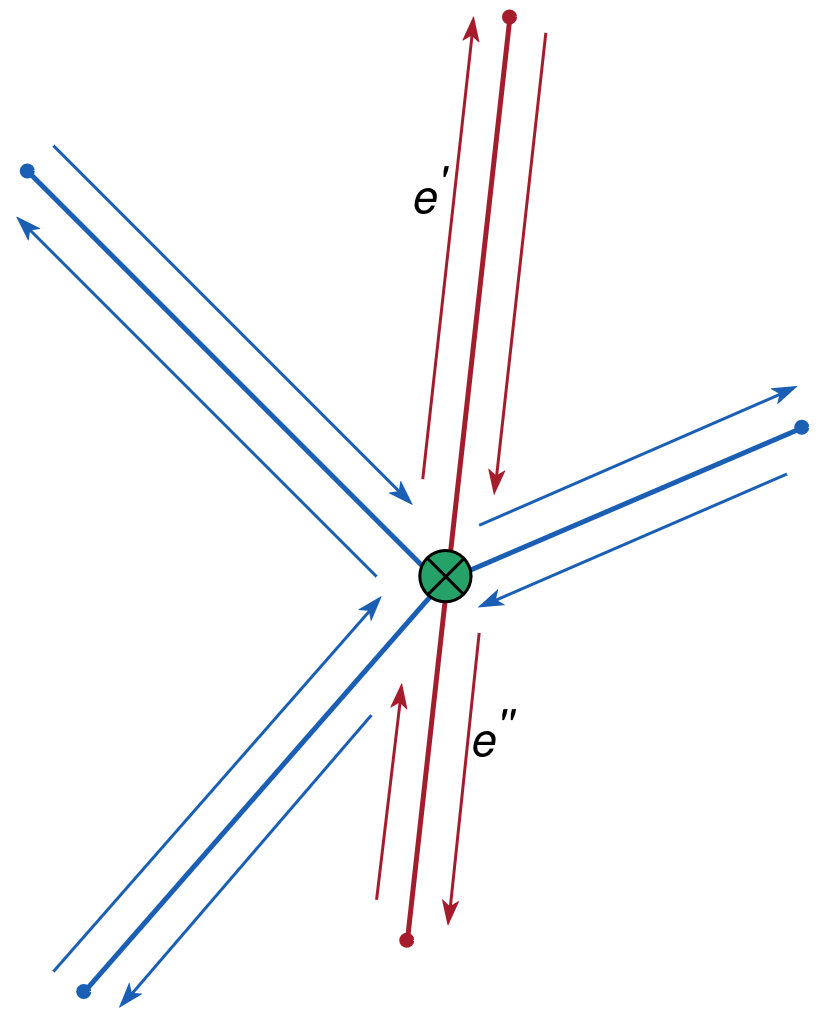
\includegraphics[width=0.9\textwidth]{images/int1.png}
\end{minipage}
\break

\begin{minipage}{0.3\textwidth}
    \centering
    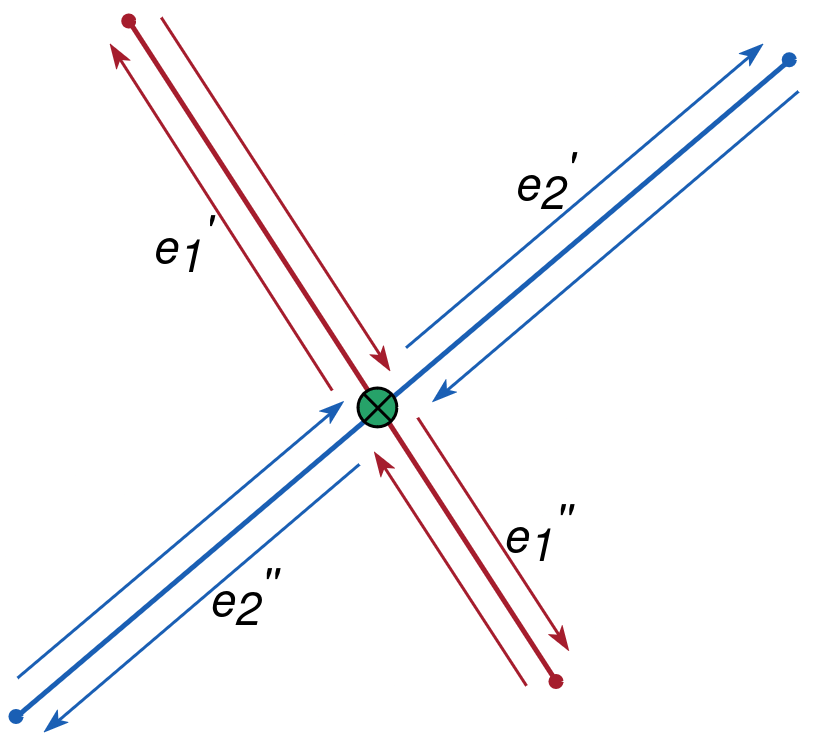
\includegraphics[width=0.9\textwidth]{images/int2.png}
\end{minipage}\hfill
\begin{minipage}{0.7\textwidth}
    We need to split both edges $e_1$ and $e_2$ into two half-edges and add a new vertex $v$ to the DCEL which has as incident edges the new four split half-edges $e_1^{\prime}$, $e_1^{\prime\prime}$, $e_2^{\prime}$ and $e_2^{\prime\prime}$. The pointers around the endpoints of the original edges $e_1$ and $e_2$ must be updated as in the previous case.
\end{minipage}
\break

\begin{minipage}{0.7\textwidth}

    After the intersection points have been processed, we need to reconstruct the faces by traversing the boundary cycles. We can do this by traversing the edges of the DCEL starting from an arbitrary edge and following the next pointers until we reach the starting edge again. This process can be repeated until all edges have been visited and all faces have been reconstructed.

    We still need to decide if the faces found are the outer faces or holes. We can do this by checking the angle of the leftmost edge of the face with the horizontal axis.  If this angle is smaller than $180^{\circ}$ then the cycle is an outer boundary, and otherwise it is the boundary of a hole.

\end{minipage}
\begin{minipage}{0.3\textwidth}
    \centering
    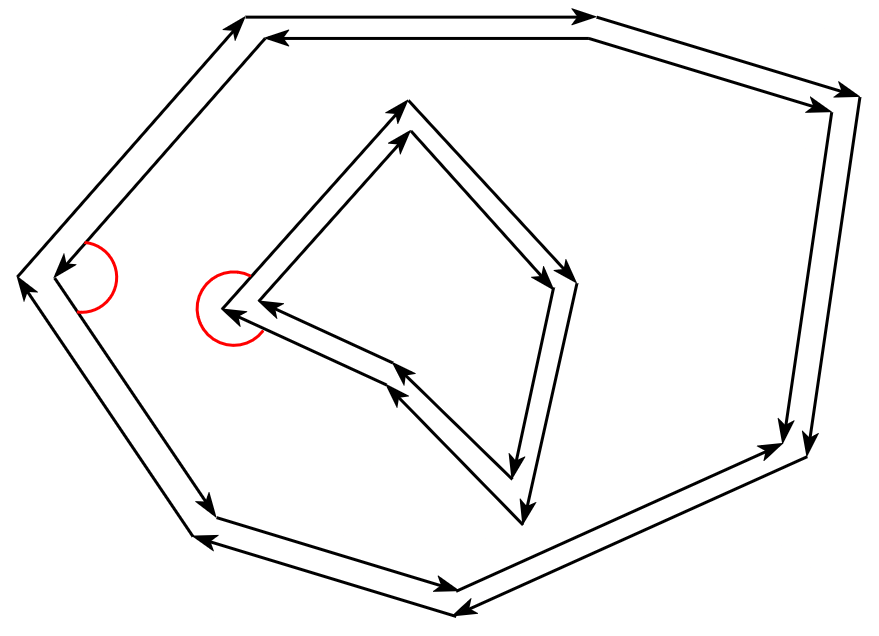
\includegraphics[width=0.9\textwidth]{images/hole.png}
\end{minipage}
\break

In order to decide which boundary cycles bound the same face, we construct a graph where each each boundary, including the one for the unbounded face, is a node and there is an edge between two nodes if and only if one of the cycles is the boundary of a hole and the other cycle has a half-edge immediately to the left of the leftmost vertex of that hole cycle. We can then find the connected components of this graph and assign the same face to all the cycles in the same component.

The last step is to label each face of the overlay with the attributes of the faces for the input subdivisions that intersect in that face.

The time complexity of this algorithm is $O((n)\log(n) + k \log(n))$ where $n = n_1 + n_1$ is the total number of edges in the two input subdivisions and $k$ is the number of intersections between edges of the two subdivisions.
